\documentclass[
  11pt,
  letterpaper,
   addpoints,
   answers
  ]{exam}
\usepackage{../exercise-preamble}
\usepackage{float}
\usepackage{subcaption}
\usepackage{circuitikz}  % tal como ya lo tienes
\ctikzset{current/american}


\begin{document}

\noindent
\begin{minipage}{0.47\textwidth}

\includegraphics[width=\textwidth]{../fcfm_die}
\end{minipage}
\begin{minipage}{0.53\textwidth}
\begin{center} 
\large\textbf{Circuitos Eléctricos Analógicos} (EL3202-1) \\
\large\textbf{Clase auxiliar 4} \\
\normalsize Prof.~ Patricio Mendoza.\\
\normalsize Prof.~Aux.~Renato Planas ~Erik Sáez
\end{center}
\end{minipage}

\vspace{0.5cm}
\noindent
\vspace{.85cm}

\begin{questions}
%----------------------------
\question
Para el circuito de la Figura~\ref{fig:1}, si utiliza la expresión exacta $I(v_D)$ del diodo, plantee la ecuación que se debe satisfacer. Plantee un modelo de aproximación para el diodo que permita resolver los voltajes y corrientes en el circuito. Sea explícito en los modelos y supuestos utilizados.
\begin{equation}
  i_D = I_s \left( e^{v_D/(\eta V_T)} - 1 \right)
\end{equation}

\begin{figure}[H]
    \centering
    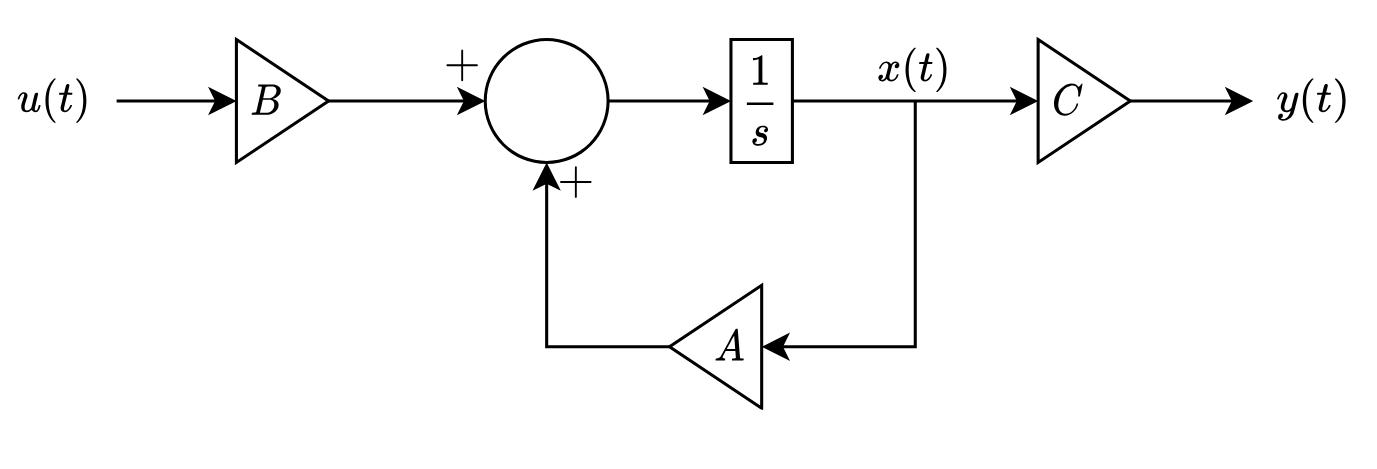
\includegraphics[width=0.8\textwidth]{Auxiliar_4_1}
    \caption{Circuito con diodo.}
    \label{fig:1}
\end{figure}
%----------------------------
\newpage
\begin{solution}
Un diodo es un dispositivo semiconductor que permite el paso de corriente en una sola dirección y presenta caracteristicas no lineales. La curva $v$ -- $i$ se puede visualizar en la figura \ref{fig:th_norton_1}:
\begin{figure}[H]
    \centering
    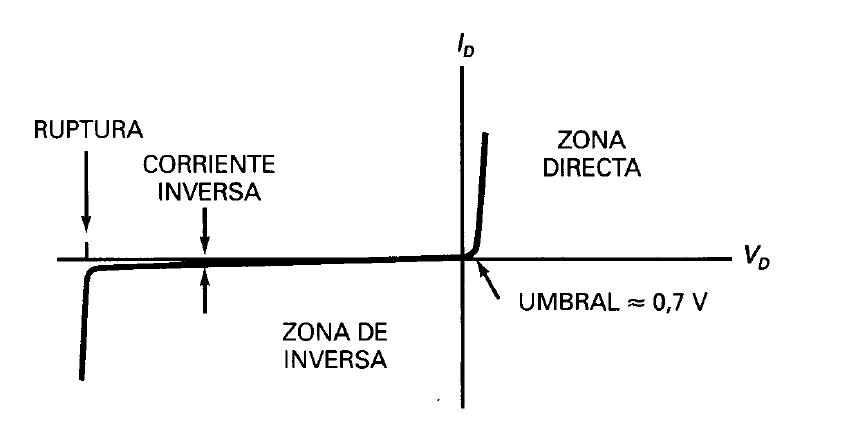
\includegraphics[width=0.8\textwidth]{Auxiliar_4_27}
  \caption{Característica $v$--$i$ del diodo. Se observa la zona directa, donde para $v_D > 0{,}7\,$V (diodo de silicio) la corriente $i_D$ crece rápidamente y el diodo conduce; el umbral de conducción cerca de $0{,}7\,$V; la zona inversa, donde para $v_D < 0$ la corriente es muy pequeña (corriente inversa de saturación); y la zona de ruptura, donde si el voltaje inverso supera un valor crítico, la corriente inversa aumenta bruscamente. Estas regiones son fundamentales para el análisis de circuitos con diodos.}
    \label{fig:th_norton_1}
\end{figure}
Ademas tenemos que la curva $v$ -- $i$ depende fuertemente de la temperatura a la cual estemos operando. Por otro lado la curva que modela el comportamiento del diodo viene dado por la ecuación de Shockley,
\begin{align}
    i_D &= I_s\left(e^{\frac{v_D}{\eta V_T}} - 1\right) 
\end{align}
Donde cada termino corresponde a:
\begin{itemize}
    \item $i_D$: corriente a través del diodo.
    \item $I_s$: corriente de saturación del diodo.
    \item $v_D$: voltaje a través del diodo.
    \item $\eta$: factor de idealidad del diodo el cual toma en cuenta las propiedades del material y para un caso ideal $\eta = 1$.
    \item $V_T$: voltaje térmico, que depende de la temperatura.
\end{itemize}
% Explicación adicional sobre el factor de idealidad
El factor de idealidad $\eta$ toma valores típicos entre 1 y 2. Un valor \(\eta\approx 1\) corresponde a un comportamiento cercano al ideal (dominancia de difusión), mientras que \(\eta\approx 2\) indica efectos no ideales —por ejemplo, recombinación de portadores en la región de agotamiento— que hacen que la corriente crezca menos rápidamente con el voltaje aplicado. En este ejercicio se considera \(\eta=2\) según el enunciado.
El denominado punto de operación del diodo corresponde al estado definido por la corriente y el voltaje que lo atraviesan. Este punto se determina por la intersección entre la curva característica $v$--$i$ del diodo y la recta de carga del circuito externo. La recta de carga expresa la relación entre voltaje y corriente impuesta por el resto del circuito, y su intersección con la característica del diodo establece el punto de operación, es decir, las condiciones reales de funcionamiento del dispositivo.

Volviendo al enunciado en este ejercicio se empleará la expresión exacta del diodo (ecuación de Shockley) evaluada a temperatura ambiente. Tomamos el voltaje térmico $V_T=25\,\mathrm{mV}$, por lo que la ecuación que describe el comportamiento del diodo es:
\begin{align}
    i_D &= I_s\left(e^{\frac{v_D}{\eta V_T}} - 1\right) \label{eq:shockley}\\
    &= 10^{-5}\,\mathrm{mA}\left(e^{\frac{v_D}{2 \cdot 25\,\mathrm{mV}}} - 1\right)\\
    &=10^{-5}\,\mathrm{mA}\big(e^{20\,v_{D}}-1\big)
\end{align}
donde $I_s$ es la corriente de saturación. En este ejercicio se considera $\eta = 2$ según el enunciado. Por la Ley de Corriente de Kirchhoff (LCK) en el nodo del diodo:
\begin{align}
    i_1 &= i_2 + i_3 \\
\frac{V_i - v_D}{R_1} &= \frac{v_D}{R_2} + I_s\left(e^{\frac{v_D}{\eta V_T}} - 1\right) \label{eq:kcl}
\end{align}

\textbf{Si suponemos que $v_D = 0{,}7\,\mathrm{V}$}, el cual es un valor común para un diodo de silicio en conducción, tenemos:
\begin{align*}
    i_1 &= \frac{V_i - v_D}{R_1} = \frac{12 - 0{,}7}{10\,000}\ \mathrm{A} = 1{,}13\ \mathrm{mA} \\
    i_2 &= \frac{v_D}{R_2} = \frac{0{,}7}{10\,000}\ \mathrm{A} = 70\ \mu\mathrm{A} \\
    i_3 &= i_1 - i_2 = 1{,}06\ \mathrm{mA}
\end{align*}
Si en vez de $v_D = 0{,}7\,\mathrm{V}$ usamos $v_D = 0{,}6\,\mathrm{V}$:
\begin{align*}
    i_1 &= \frac{12 - 0{,}6}{10\,000} = 1{,}14\ \mathrm{mA} \\
    i_2 &= \frac{0{,}6}{10\,000} = 60\ \mu\mathrm{A} \\
    i_3 &= i_1 - i_2 = 1{,}08\ \mathrm{mA}
\end{align*}
Vemos que obtenemos valores bastante pequeños para la corriente del diodo, lo que puede parecer contradictorio, pero esto se debe al punto de operación en el que se encuentra el diodo. En efecto, como $i_D$ depende de $v_D$, al fijar a priori un valor (p.\,ej., $0{,}6$–$0{,}7\,\mathrm{V}$) estamos usando un \emph{modelo de caída constante}; así, $i_3=i_1-i_2$ es consistente con esa suposición, pero no necesariamente con la ecuación de Shockley. Para hallar el punto de operación coherente con el modelo exacto debe resolverse por $v_D$ la ecuación no lineal
\[
g(v_D)\equiv \frac{V_i-v_D}{R_1}-\frac{v_D}{R_2}-I_s\!\left(e^{\frac{v_D}{\eta V_T}}-1\right)=0,
\]
y luego calcular $i_1$, $i_2$ e $i_D$ con ese $v_D^\star$, cumpliéndose exactamente $i_D=i_1-i_2$. En este circuito se obtiene numéricamente $v_D^\star\approx 0{,}58\,\mathrm{V}$, $i_1\approx 1{,}142\,\mathrm{mA}$, $i_2\approx 0{,}058\,\mathrm{mA}$ e $i_D\approx 1{,}084\,\mathrm{mA}$, lo que explica por qué imponer $v_D=0{,}6$–$0{,}7\,\mathrm{V}$ sobrestima el voltaje directo o no cuadra con la recta de carga. Ahora analizaremos dos situaciones límite para el diodo:
\begin{itemize}
  \item \textbf{Caso 1: diodo en corte ($i_D=0$).} El diodo no conduce y equivale a un circuito abierto; sólo circula corriente por $R_1$ y $R_2$ en serie:
  \begin{figure}[H]
    \centering
    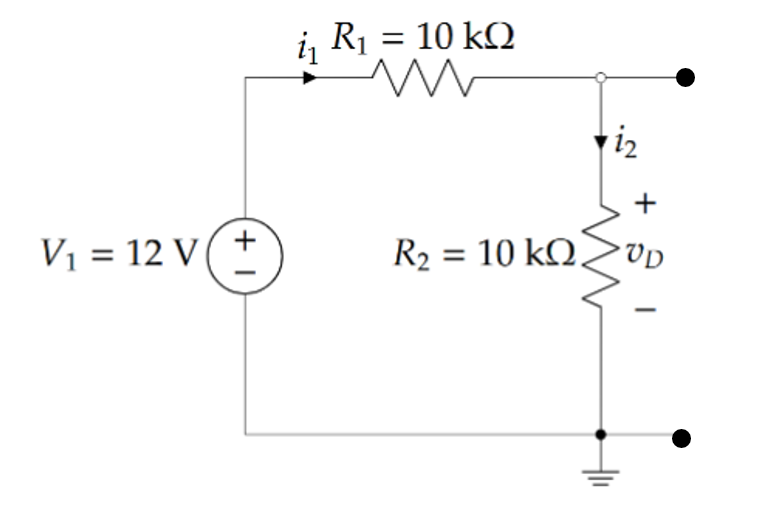
\includegraphics[width=0.4\textwidth]{Auxiliar_4_10}
    \caption{Circuito con el diodo abierto.}
    \label{fig:th_norton_2}
  \end{figure}
  \vspace{-0.6em}
  \[
    12 = (R_1+R_2)\,i
    \;\;\Rightarrow\;\;
    i=\frac{12}{20\,000}=0{,}6~\mathrm{mA},
    \qquad
    v_D = i\,R_2 = 6~\mathrm{V}.
  \]
  Es decir, el eje $v_D$ corta a la recta de carga en $v_D=6~\mathrm{V}$ cuando $i_D=0$.

  \item \textbf{Caso 2: diodo en conducción (cortocircuito ideal).} El diodo se modela como un corto; el nodo queda forzado a $v_D=0$ y por $R_2$ no circula corriente:
  \begin{figure}[H]
    \centering
    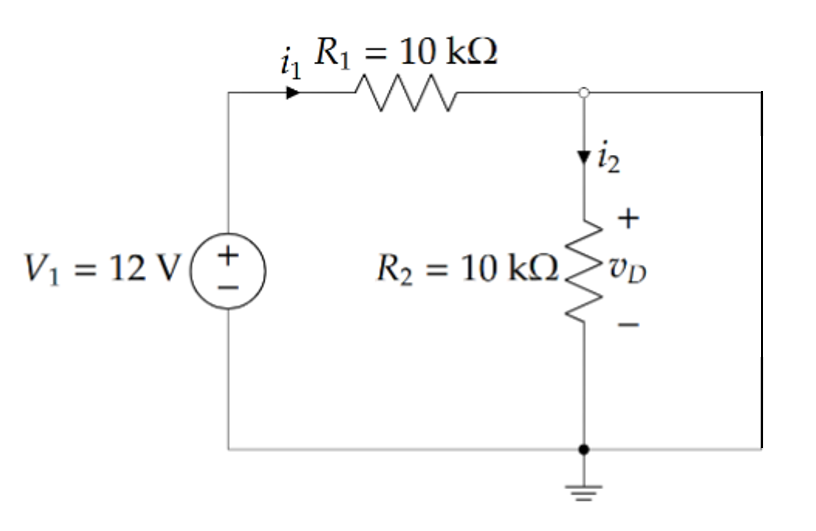
\includegraphics[width=0.4\textwidth]{Auxiliar_4_11}
    \caption{Circuito con el diodo en cortocircuito.}
    \label{fig:th_norton_3}
  \end{figure}
  \vspace{-0.6em}
  \[
    12 = R_1\,i
    \;\;\Rightarrow\;\;
    i=\frac{12}{10\,000}=1{,}2~\mathrm{mA},
    \qquad
    v_D=0.
  \]
  Así, el eje $i_D$ corta a la recta de carga en $i_D=1{,}2~\mathrm{mA}$ cuando $v_D=0$.
\end{itemize}

Los dos casos límite anteriores fijan los \emph{interceptos} de la recta de carga del circuito externo en el plano $(v_D,i_D)$. Para cualquier $v_D\in[0,6]~\mathrm{V}$, la relación impuesta por $R_1$ y $R_2$ viene dada por
\[
  i_D \;=\; \frac{V_i - v_D}{R_1} \;-\; \frac{v_D}{R_2},
\]
que es precisamente la \emph{recta de carga} (pasa por los puntos $(v_D,i_D)=(0,1{,}2~\mathrm{mA})$ y $(6~\mathrm{V},0)$).
La intersección entre esta recta y la característica no lineal del diodo \eqref{eq:shockley} determina el \emph{punto de operación}. En este circuito, dicha intersección ocurre para un voltaje directo algo menor que $0{,}6~\mathrm{V}$ (numéricamente, $\approx 0{,}58~\mathrm{V}$), por lo que, debido al crecimiento exponencial de \eqref{eq:shockley}, la corriente de operación resulta del orden de los miliamperes. Para desplazar el punto de operación hacia corrientes mayores sería necesario \emph{endurecer} la recta de carga (por ejemplo, disminuyendo $R_1$ y/o $R_2$ o aumentando $V_i$).

\begin{figure}[H]
  \centering
  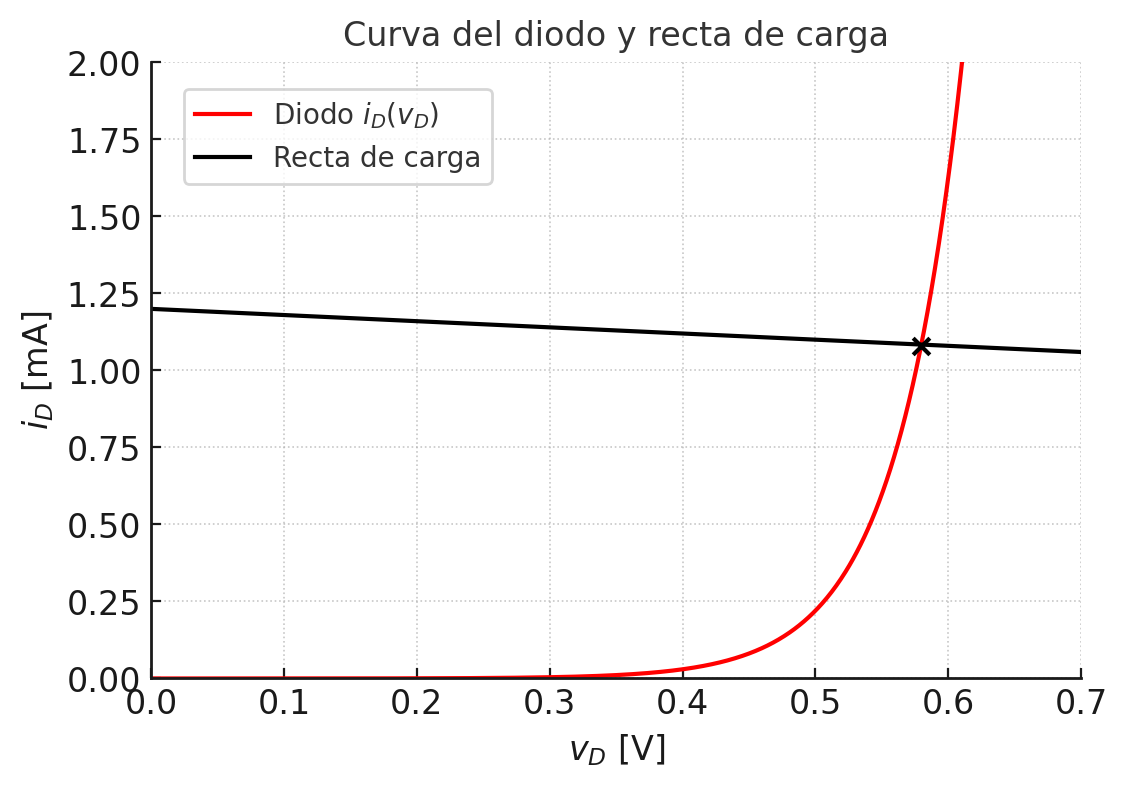
\includegraphics[width=0.6\textwidth]{Auxiliar_4_2}
  \caption{Punto de operación: intersección entre la característica $v$–$i$ del diodo y la recta de carga del circuito.}
  \label{fig:th_norton_6}
\end{figure}
Entonces, de manera visual, el punto de intersección (punto de operación) queda aproximadamente en:
\begin{align}
  v_D^\star &\approx 0{,}58~\mathrm{V}, &
  i_D^\star &\approx 1{,}08~\mathrm{mA}.
\end{align}
Los cuales son los mismos obtenidos con anterioridad.
\end{solution}

%----------------------------
    \question Un diodo Zener con característica $v$--$i$, como la mostrada en la Figura 5a), tiene un voltaje de Zener
    $V_{ZK}=3\ \mathrm{V}$. Determine la corriente $i_X$ en los dos circuitos mostrados en la figura \ref{fig:ex4c}. Sea explícito en los modelos y supuestos utilizados.  

% --- Figuras de los dos casos ---
\begin{figure}[H]
  \centering

  \begin{subfigure}[b]{0.48\textwidth}
    \centering
    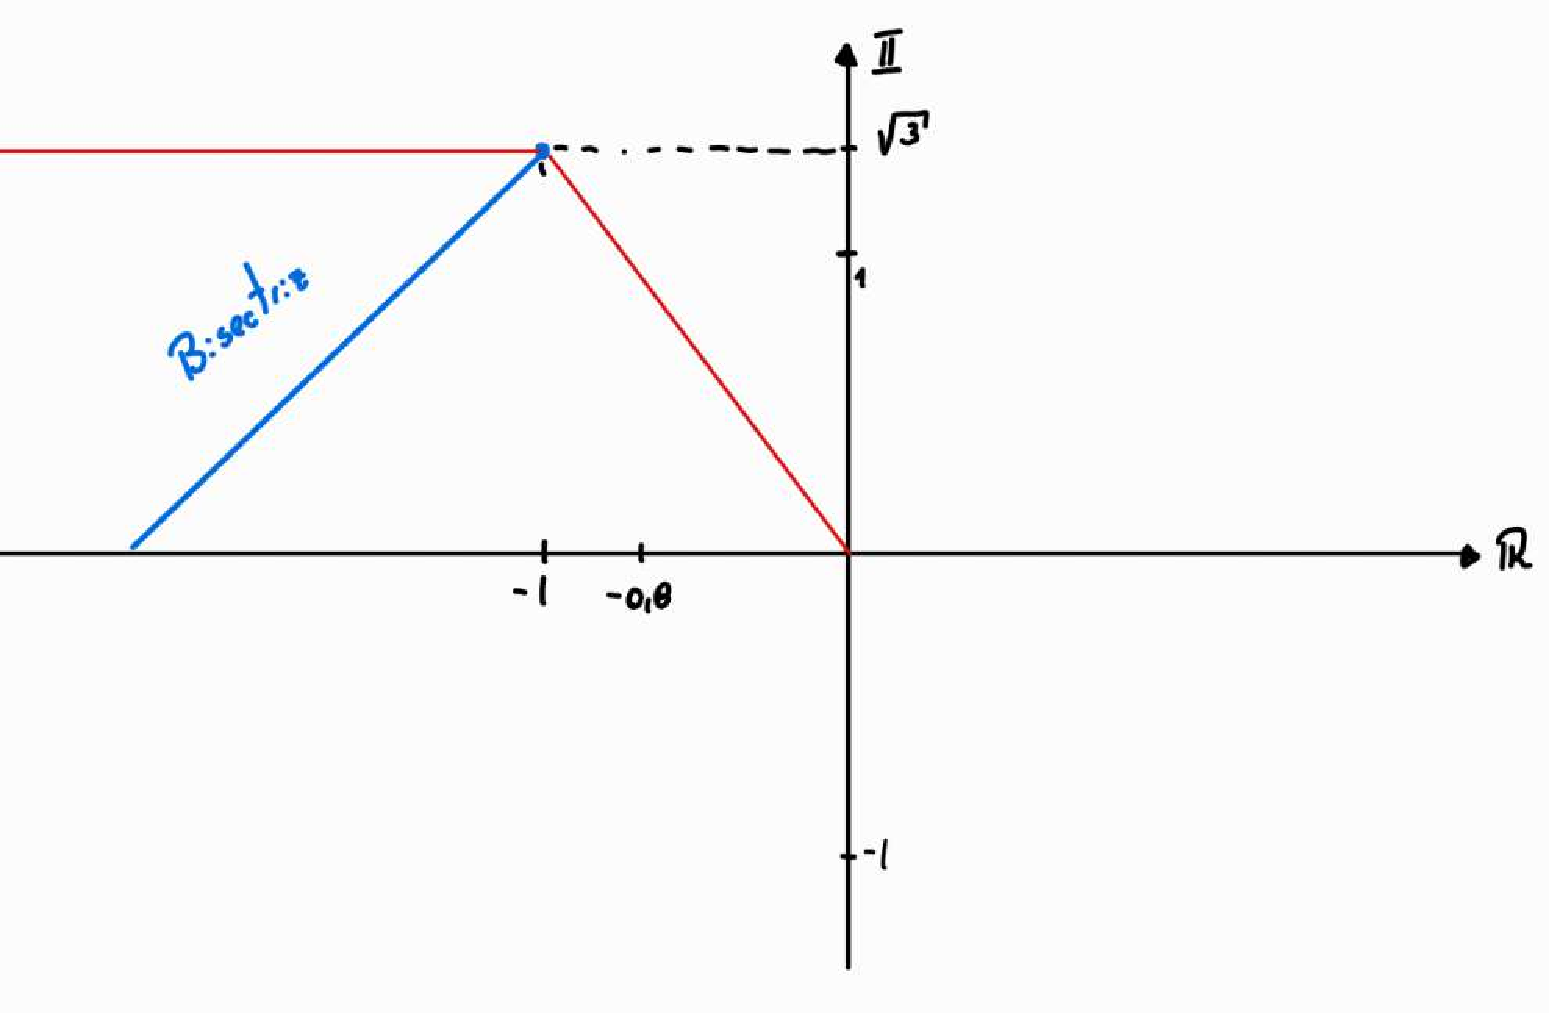
\includegraphics[width=1\linewidth]{Auxiliar_4_5}
    \caption{Curva de v-i del diodo Zener.}
    \label{fig:ex4a}
  \end{subfigure}\hfill
  \begin{subfigure}[b]{0.48\textwidth}
    \centering
    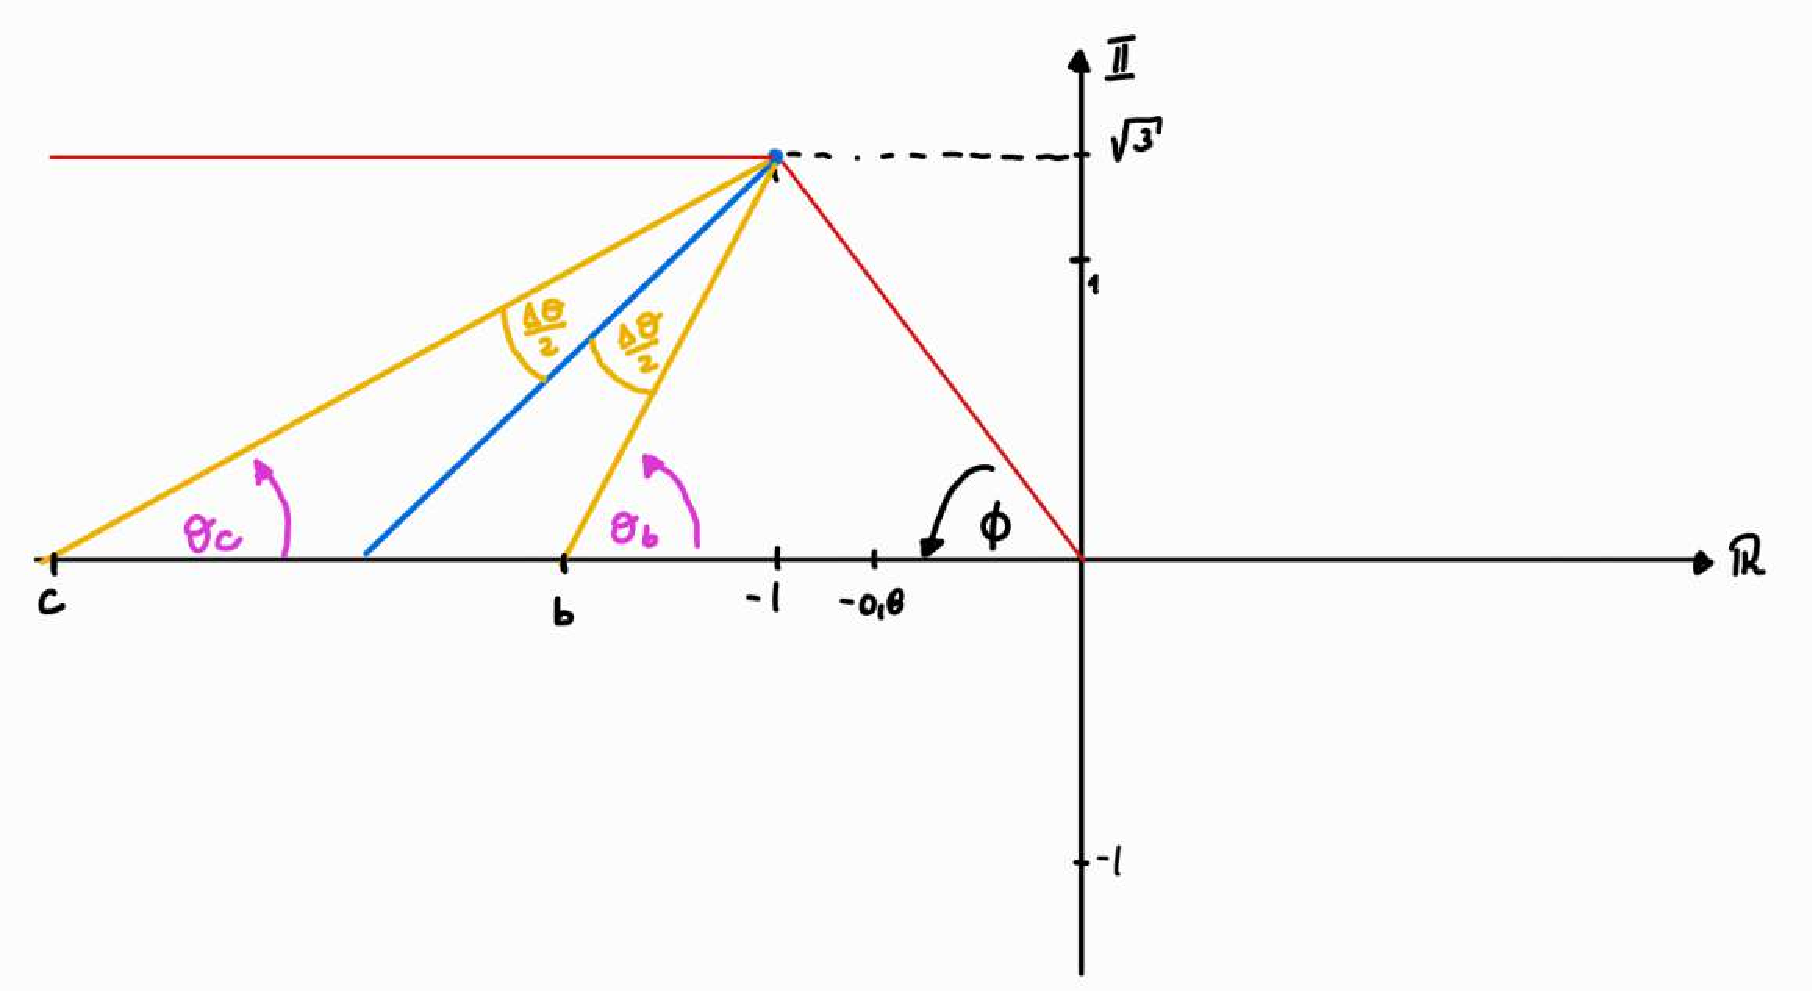
\includegraphics[width=0.5\linewidth]{Auxiliar_4_6}
    \caption{Esquema de un diodo Zener.}
    \label{fig:ex4b}
  \end{subfigure}

  \caption{ (a) Característica $v$--$i$ del diodo Zener, mostrando las regiones de polarización directa, inversa y de ruptura inversa, así como los valores típicos de voltaje y corriente. (b) Símbolo del diodo Zener, mostrando la dirección de la corriente $i_Z$ y el voltaje $v_Z$ en sus terminales.}
  \label{fig:ex4ab}
\end{figure}


\begin{figure}[H]
  \centering  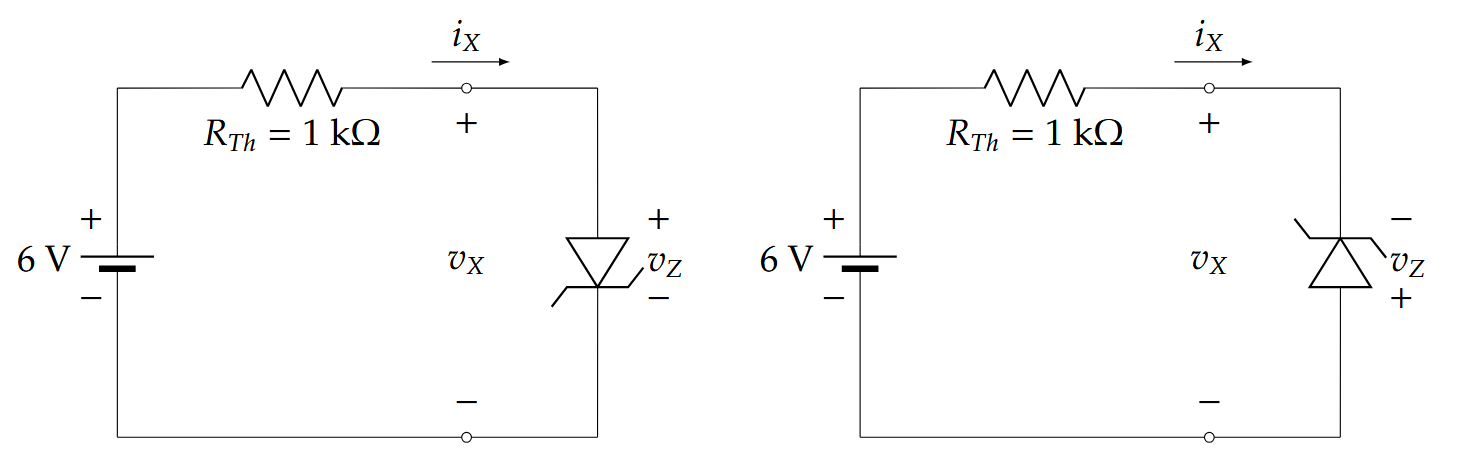
\includegraphics[width=0.9\textwidth]{Auxiliar_4_7}
  \caption{Detalle: (izquierda) símbolo del diodo Zener con convención de corriente $i_Z$ y polaridad de $v_Z$; (derecha) característica $v$--$i$ esquemática del diodo (ruptura inversa alrededor de $-V_{ZK}$).}
  \label{fig:ex4c}
\end{figure}


%----------------------------

\begin{solution}
Similar a lo anterior, el primer paso es trazar la \emph{recta de carga} del equivalente de Thévenin (fuente de $6~\text{V}$ en serie con $R_{\text{Th}}=1~\text{k}\Omega$). Por lo que primeramente nos centramos en sus interceptos se obtienen de:
\begin{align}
i_X&=0 \;\Rightarrow\; v_X=6~\text{V},\\
v_X&=0 \;\Rightarrow\; i_X=\frac{6}{1\,000}=6~\text{mA}.
\end{align}
Luego obtenemos mediante los dos puntos anteriores la recta de carga del circuito externo:
\begin{align}
i_X \;=\; \frac{6-v_X}{R_{\text{Th}}}
\;=\; \frac{6-v_X}{1\,000}.
\end{align}
En el circuito de la Figura~\ref{fig:carac-v-i}, aproximamos la característica del diodo por tramos:
\begin{align*}
&\text{Directa:}\quad v_X>0{,}7~\text{V}\;\Rightarrow\; v_Z \approx 0{,}7~\text{V},\\
&\text{Ruptura:}\quad v_X<-3~\text{V}\;\Rightarrow\; v_Z \approx -3~\text{V}.
\end{align*}
Bajo la hipótesis de que la fuente tiene un valor de  $0{,}7$ V en directa, la corriente de operación resulta 
\begin{align}
i_X \;=\; \frac{6-0{,}7}{1\,000} \;=\; 5{,}3~\text{mA},
\end{align}
valor que coincide, dentro de la aproximación, con el cruce visual entre la recta de carga y la curva del diodo.

\begin{figure}[H]
  \centering
  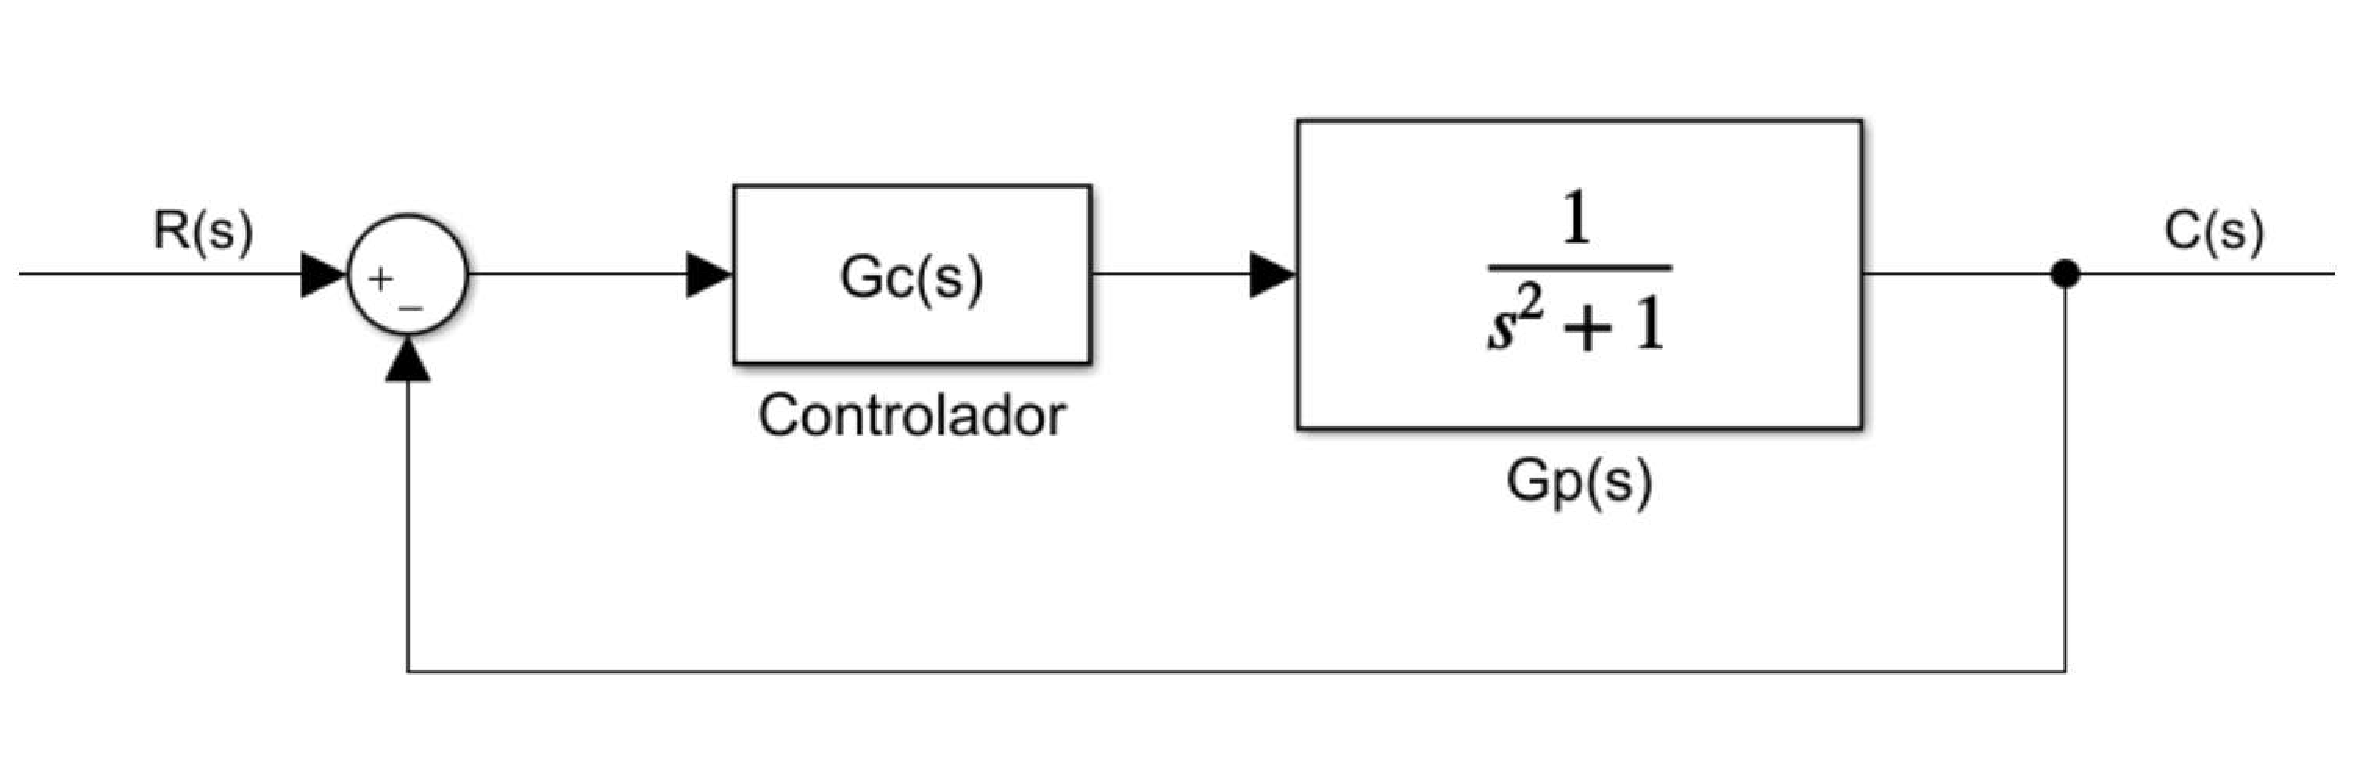
\includegraphics[width=0.5\textwidth]{Auxiliar_4_8}
  \caption{Curva $v$--$i$ del voltaje $v_X$ (azul) y recta de carga del equivalente (verde). Ejes: $v_X$ (V) horizontal e $i_X$ (mA) vertical. Los interceptos de la recta en este ejemplo son $v_X=6\,$V e $i_X=6\,$mA. La intersección curva/recta fija el punto de operación: en la región directa $v\approx V_f\simeq0{,}7\,$V, en la región de ruptura el voltaje queda próximo a $-V_{ZK}$. Cambiar $R_{\text{Th}}$ o la fuente desplaza la recta y, por tanto, el punto de operación.}
  \label{fig:carac-v-i}
\end{figure}


Para el circuito de la derecha (Figura~\ref{fig:iv-diodo}), con el Zener invertido, la región relevante es la de \emph{ruptura inversa}:
\begin{align*}
&\text{Ruptura:}\quad v_X>3~\text{V}\;\Rightarrow\; v_Z \approx -3~\text{V},\\
&\text{Directa:}\quad v_X<0{,}7~\text{V}\;\Rightarrow\; v_Z \approx 0{,}7~\text{V}.
\end{align*}
Adoptando el modelo de \emph{fuente de \(-3\) V} en ruptura,
\begin{align}
i_X \;=\; \frac{6-3}{1\,000} \;=\; 3~\text{mA},
\end{align}
en concordancia con el punto de intersección observado en la gráfica (tener presente la convención de signos: el Zener está invertido, por lo que en la figura la región de ruptura aparece hacia $+v_X$ y la corriente cambia de signo).

\begin{figure}[H]
  \centering
  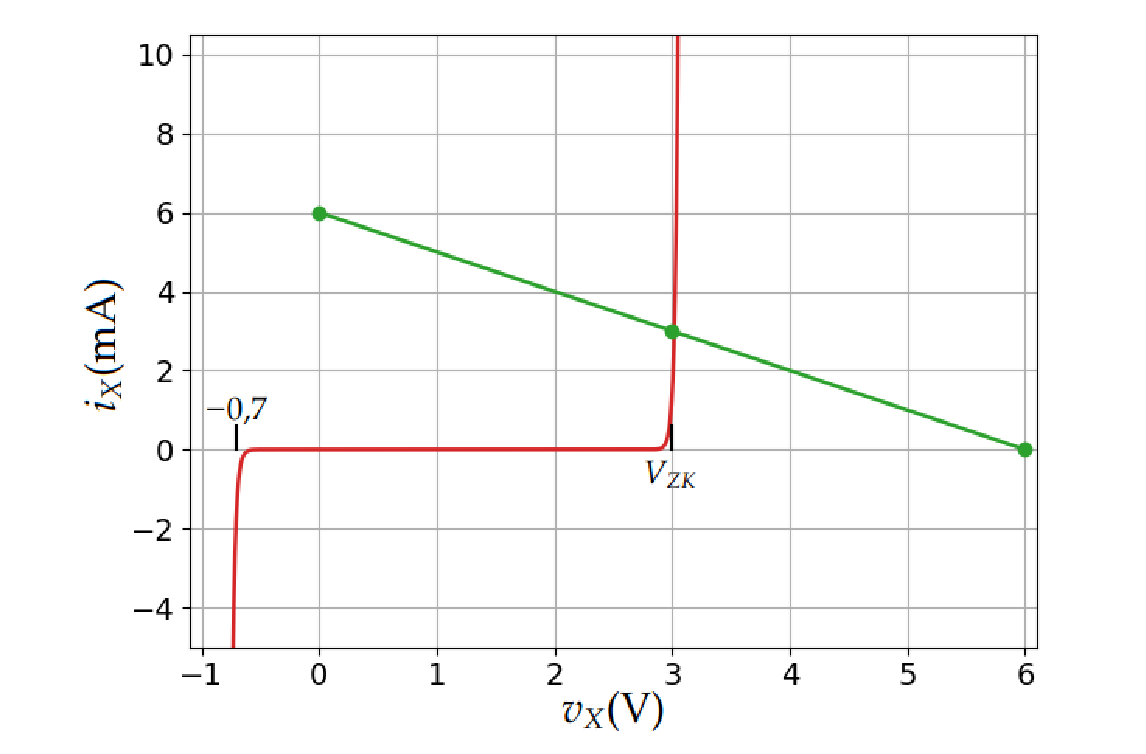
\includegraphics[width=0.5\textwidth]{Auxiliar_4_9}
  \caption{Característica $v$--$i$ de $v_X$ (azul) y recta de carga (verde) para el circuito con Zener invertido. Ejes: $v_X$ (V) horizontal e $i_X$ (mA) vertical. En ruptura inversa el diodo mantiene $v_X\approx -V_{ZK}$ (aquí $V_{ZK}=3\,$V) y la recta de carga intersecta dicha rama dando $i_X\approx3\,$mA en el ejemplo mostrado.}
  \label{fig:iv-diodo}
\end{figure}
\end{solution}

%----------------------------

\question Para el circuito de la figura \ref{fig:3}, bosqueje el voltaje en el diodo y la corriente en el diodo como función del tiempo. Sea explícito en los valores de las gráficas, así como en los modelos y supuestos utilizados.
\begin{figure}[H]
  \centering
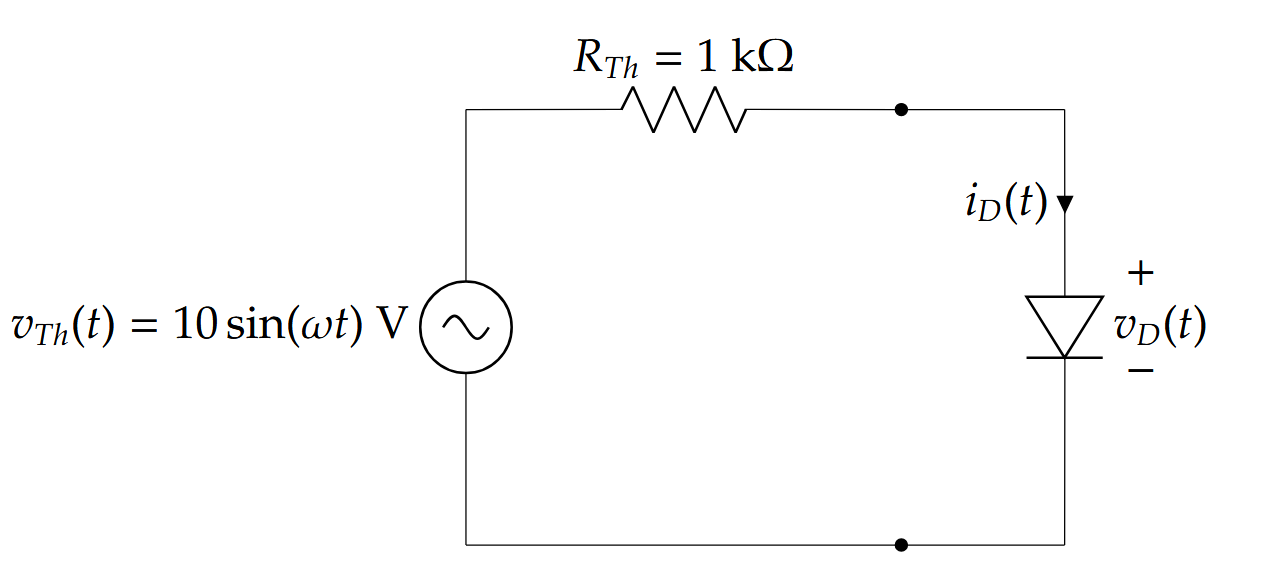
\includegraphics[width=0.7\textwidth]{Auxiliar_4_12}
  \caption{Circuito con diodo y fuente de voltaje senoidal.}
  \label{fig:3}
\end{figure}
%----------------------------

\begin{solution}
Para clarificar el funcionamiento con $v_{\text{Th}}(t)=10\sin(\omega t)\,[\text{V}]$ y $R_{\text{Th}}=1~\text{k}\Omega$, usaremos el modelo por tramos del diodo:
\begin{align}
\text{Directa (ON):}\quad &v_D(t)\approx V_f\simeq 0{,}7~\text{V}, & i_D(t)\approx \frac{v_{\text{Th}}(t)-V_f}{R_{\text{Th}}}\ \ (\ge 0),\\
\text{Inversa (OFF):}\quad &i_D(t)\approx -I_s\approx 0, & v_D(t)\approx v_{\text{Th}}(t),
\end{align}
El diodo entra en conducción cuando $v_{\text{Th}}(t)\ge V_f$. Con este criterio, evaluamos algunos instantes clave del ciclo (nótese que en inversa hemos dejado $\approx -I_s$ para resaltar que es \emph{muy} pequeña frente a los mA en directa):
\begin{table}[H]
  \centering
  \begin{tabular}{c c c c c c}
    \hline
    Punto de operación & $\omega t$ & $\sin(\omega t)$ & $v_{\text{Th}}(t)$ (V) & $v_D$ (V) & $i_D$ (mA) \\
    \hline
    3 & $0$ & $0$ & $0$ & $0$ & $0$ \\
    2 & $\pi/6$ & $1/2$ & $5$ & $0.7$ & $\dfrac{5-0.7}{1000}=4.3$ \\
    1 & $\pi/2$ & $1$ & $10$ & $0.7$ & $\dfrac{10-0.7}{1000}=9.3$ \\
    2 & $5\pi/6$ & $1/2$ & $5$ & $0.7$ & $4.3$ \\
    3 & $\pi$ & $0$ & $0$ & $0$ & $0$ \\
    4 & $7\pi/6$ & $-1/2$ & $-5$ & $-5$ & $\approx -I_s\ (\approx 0)$ \\
    5 & $3\pi/2$ & $-1$ & $-10$ & $-10$ & $\approx -I_s\ (\approx 0)$ \\
    4 & $11\pi/6$ & $-1/2$ & $-5$ & $-5$ & $\approx -I_s\ (\approx 0)$ \\
    3 & $2\pi$ & $0$ & $0$ & $0$ & $0$ \\
    \hline
  \end{tabular}
  \caption{Valores de voltaje y corriente en el diodo para distintos puntos de operación durante un ciclo senoidal.}
  \label{tab:diodo-operacion}
\end{table}
a variación del punto de operación con el tiempo se visualiza en:
\begin{figure}[H]
    \centering
    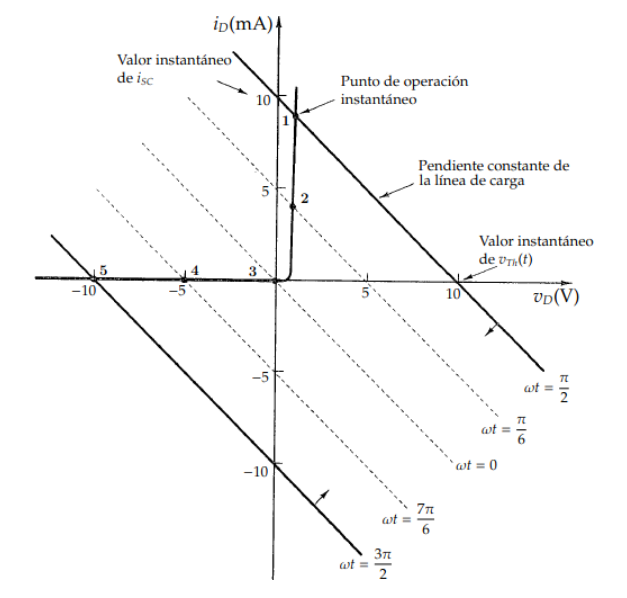
\includegraphics[width=0.5\textwidth]{Auxiliar_4_17}
    \caption{Voltaje de Thévenin $v_{\text{Th}}(t)=10\sin(\omega t)$ como función del tiempo.}
    \label{fig:voltaje-th}
\end{figure}

\noindent Dependiendo del signo y magnitud instantánea de $v_{\text{Th}}(t)$, el circuito se reduce a:
\begin{figure}[H]
  \centering
  \begin{subfigure}[b]{0.45\textwidth}
    \centering
    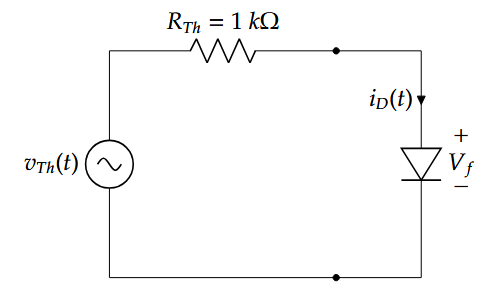
\includegraphics[width=0.8\linewidth]{Auxiliar_4_13}
    \caption{Diodo abierto ($i_D(t)\approx 0$) cuando $v_{\text{Th}}(t)<V_f$.}
    \label{fig:diodo-abierto}
  \end{subfigure}\hfill
  \begin{subfigure}[b]{0.4\textwidth}
    \centering
    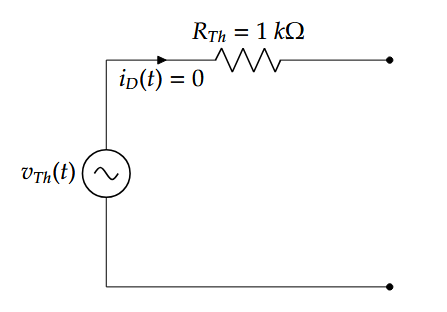
\includegraphics[width=0.8\linewidth]{Auxiliar_4_14}
    \caption{Diodo conduciendo ($v_D\approx V_f$) cuando $v_{\text{Th}}(t)\ge V_f$.}
    \label{fig:diodo-conduce}
  \end{subfigure}
  \caption{Modelos instantáneos del circuito con diodo.}
  \label{fig:diodo-operacion-casos}
\end{figure}
Gráficamente:
\begin{figure}[H]
  \centering
  \begin{subfigure}[b]{0.48\textwidth}
    \centering
    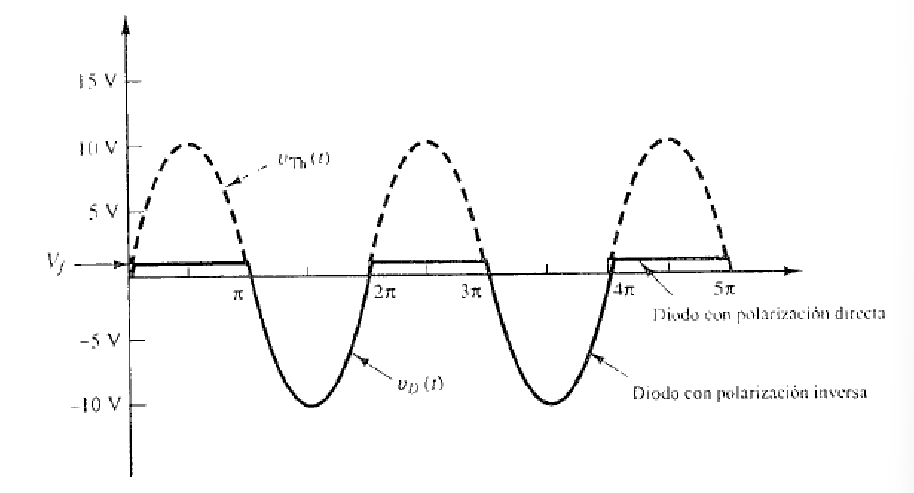
\includegraphics[width=\linewidth]{Auxiliar_4_15}
    \caption{Forma de $v_D(t)$: durante cada semionda positiva, cuando $v_{\text{Th}}(t)\ge V_f$, el diodo entra en polarización directa y el voltaje queda "recortado" cerca de la caída de conducción $V_f$ (modelo por tramos $v_D\approx V_f$); en los intervalos donde $v_{\text{Th}}(t)<V_f$ (polarización inversa) el diodo está esencialmente abierto y $v_D(t)$ sigue la tensión de la fuente $v_{\text{Th}}(t)$. En términos angulares, la conducción ocurre entre los instantes en que $10\sin(\omega t)=V_f$, y el resto del ciclo el diodo permanece bloqueado.}
    \label{fig:voltaje-corriente-diodo}
  \end{subfigure}\hfill
  \begin{subfigure}[b]{0.48\textwidth}
    \centering
    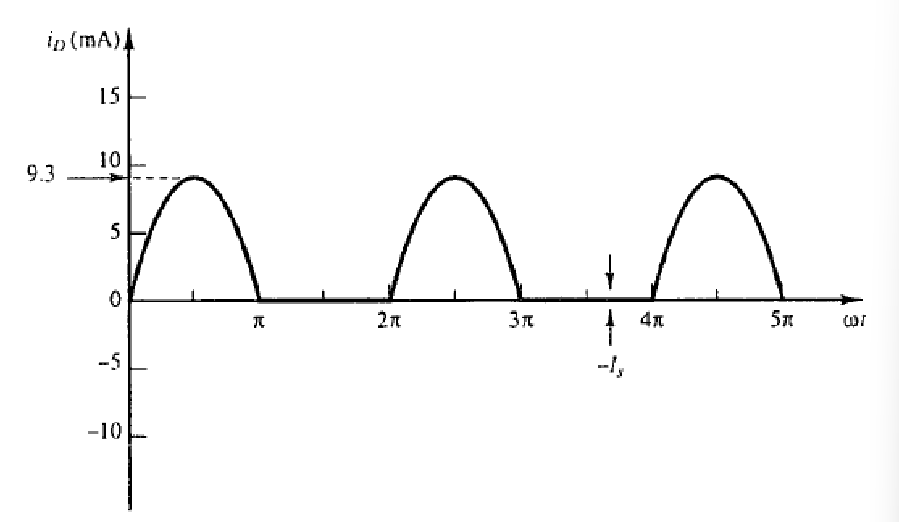
\includegraphics[width=\linewidth]{Auxiliar_4_16}
    \caption{Forma de $i_D(t)$: la corriente es apreciable sólo durante los intervalos en que la fuente supera el umbral de conducción $V_f$ (polarización directa), quedando prácticamente nula en polarización inversa (solo circula la pequeña corriente de saturación $I_s$). El pulso de corriente durante cada semionda positiva tiene forma aproximadamente parabólica cuando se considera la dependencia con $\sin(\omega t)$; su máximo se alcanza en $\omega t=\pi/2$ y, con los datos del ejercicio, valdría $i_{D,\max}=9{,}3\,$mA.}
    \label{fig:voltaje-corriente-diodo-detalle}
  \end{subfigure}
  \caption{(a) Voltaje instantáneo en el diodo $v_D(t)$ y (b) corriente en el diodo $i_D(t)$ durante un ciclo de $v_{\text{Th}}(t)=10\sin(\omega t)$. En (a) se aprecia el recorte a $V_f$ durante la conducción; en (b) se muestra el pulso de corriente correspondiente y su valor máximo.}
  \label{fig:voltaje-corriente-diodo-combined}
\end{figure}

Esta construcción coincide con el método gráfico de \emph{rectas de carga instantáneas}:
la pendiente es constante $-1/R_{\text{Th}}$ y la ordenada varía con $v_{\text{Th}}(t)$, generando los puntos de operación mostrados en la figura de referencia.

\end{solution}
%----------------------------

\question Sea el esquema visto en \ref{fig:P2_17} responda lo siguiente, considerando la fuente de voltaje que ahi aparece.
\begin{enumerate}
    \item Represente (bosqueje) \(v_o\) en función del tiempo para el circuito de la Figura~\ref{fig:P2_17} (Lado izquierdo)
    con la entrada mostrada. Suponga \(V_\gamma = 0\).
    \item \textbf{[Propuesto:]} Represente (bosqueje) \(v_o\) en función del tiempo para el circuito de la
  Figura~\ref{fig:P2_17} (Lado derecho). La entrada es senoidal y está dada por
  \(v_i(t) = 10 \sin(\omega t)\,\text{V}\). Suponga \(V_\gamma = 0\).
\end{enumerate}

\begin{figure}[H]
    \centering
    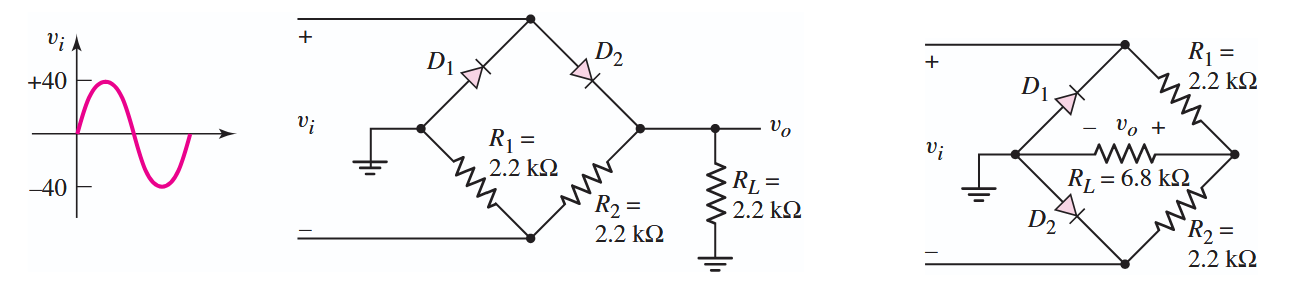
\includegraphics[width=1\textwidth]{Auxiliar_4_18}
  \caption{Esquema del circuito con diodos.}
    \label{fig:P2_17}
\end{figure}
%----------------------------

\begin{solution}
    \subsection*{Resolucion 4.1}
   
Se desea bosquejar \(v_o(t)\). Con diodos ideales (\(V_\gamma=0\)), el análisis se hace por casos según el signo de \(v_i\). En cada caso, el diodo se reemplaza por su modelo ON (corto) u OFF (abierto), como se muestra en las Figuras~\ref{fig:resolucion4.1a} y \ref{fig:resolucion4.1b}.

\begin{figure}[H]
  \centering
  \begin{subfigure}[b]{0.48\textwidth}
    \centering
    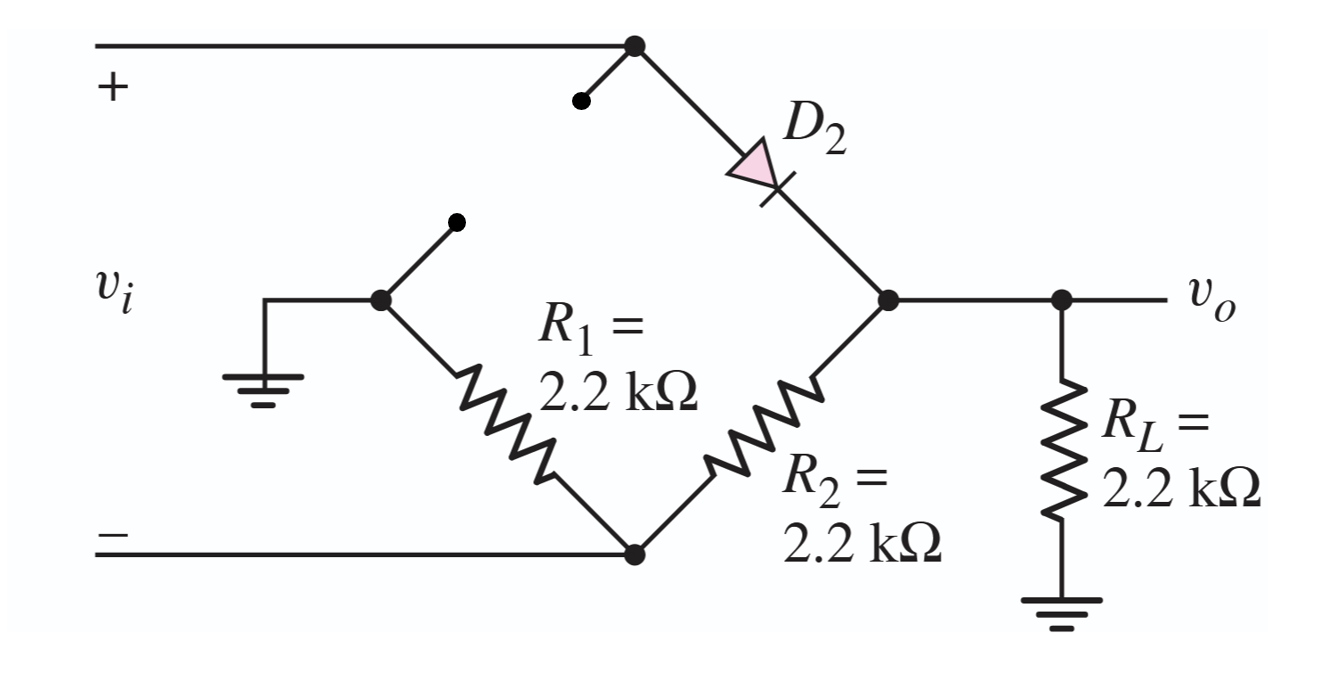
\includegraphics[width=\linewidth]{Auxiliar_4_19}
    \caption{\textbf{Caso A:} \(v_i>0\) $\Rightarrow$ \(D_1\) está OFF y \(D_2\) está ON.}
    \label{fig:resolucion4.1a}
  \end{subfigure}\hfill
  \begin{subfigure}[b]{0.48\textwidth}
    \centering
    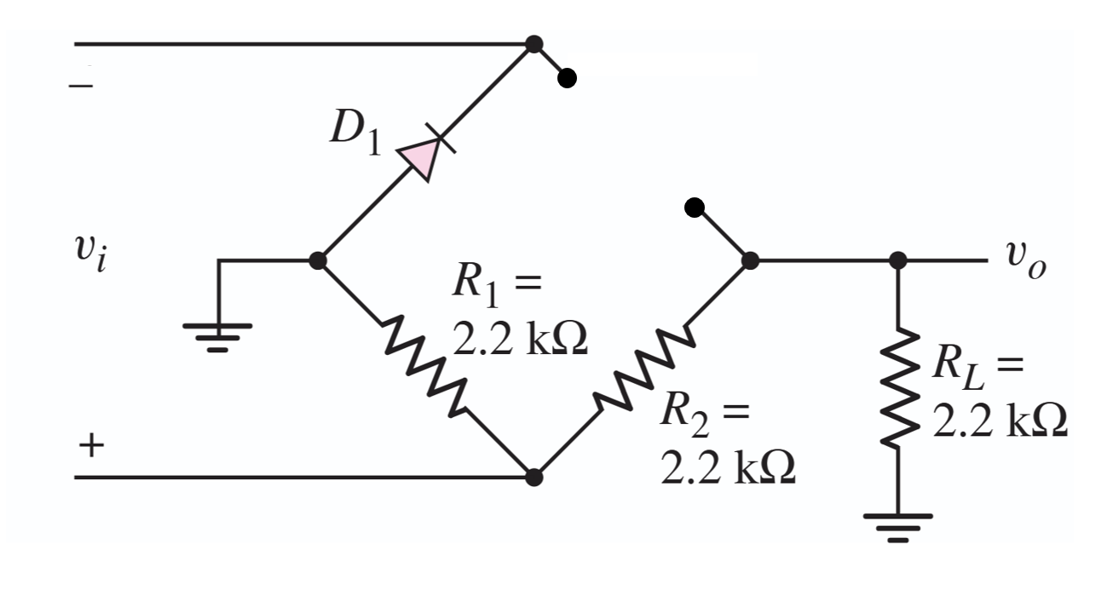
\includegraphics[width=\linewidth]{Auxiliar_4_20}
    \caption{\textbf{Caso B:} \(v_i<0\) $\Rightarrow$ \(D_1\) está ON y \(D_2\) está OFF.}
    \label{fig:resolucion4.1b}
  \end{subfigure}
  \caption{Modelo ON/OFF del diodo para cada semiciclo. En ambos casos, visto desde \(v_o\) el diagrama reducido es del mismo tipo: o bien \(v_o\) queda \emph{fijado} por la fuente (diodo ON) o bien queda \emph{aislado} de la fuente (diodo OFF) y conectado a tierra por las resistencias.}
  \label{fig:resolucion4.1}
\end{figure}

Para facilitar el equivalente, conviene \emph{etiquetar nodos} y reordenar el circuito (sin cambiar conexiones). Así se obtiene el esquema de la Figura~\ref{fig:equivalente-vo}.

\begin{figure}[H]
  \centering
  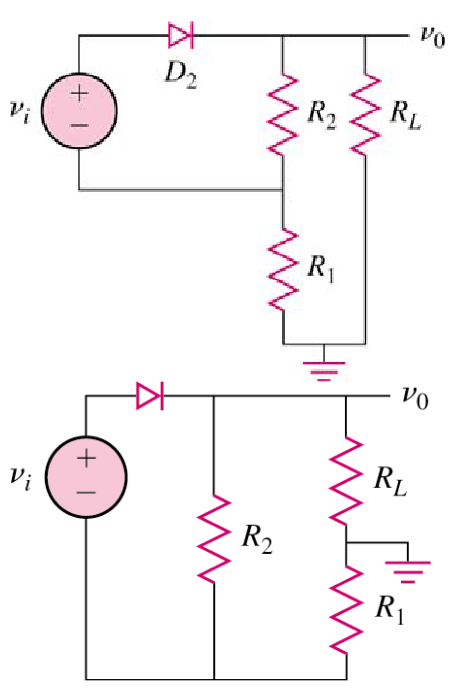
\includegraphics[width=0.30\textwidth]{Auxiliar_4_22}
  \caption{Esquema equivalente “visto” desde \(v_o\), \textbf{idéntico en ambos semiciclos}. Con el diodo ON, \(v_o\) queda fijado por la fuente (corto ideal); con el diodo OFF, \(v_o\) queda aislado de la fuente y desciende a \(0\) a través de las ramas resistivas.}
  \label{fig:equivalente-vo}
\end{figure}

La consecuencia importante es que, por simetría, la forma del circuito \emph{desde \(v_o\)} es equivalente para \(v_i>0\) y \(v_i<0\). Por ello, el nodo \(v_o\) resulta siempre no negativo: en el semiciclo positivo sigue a la fuente; en el semiciclo negativo el arreglo con el diodo opuesto produce el mismo efecto visto desde \(v_o\). Con diodos ideales y fuente ideal, esto se traduce en una \textbf{rectificación de onda completa}:
\[
v_o(t)=|\,v_i(t)\,|.
\]

\begin{figure}[H]
  \centering
  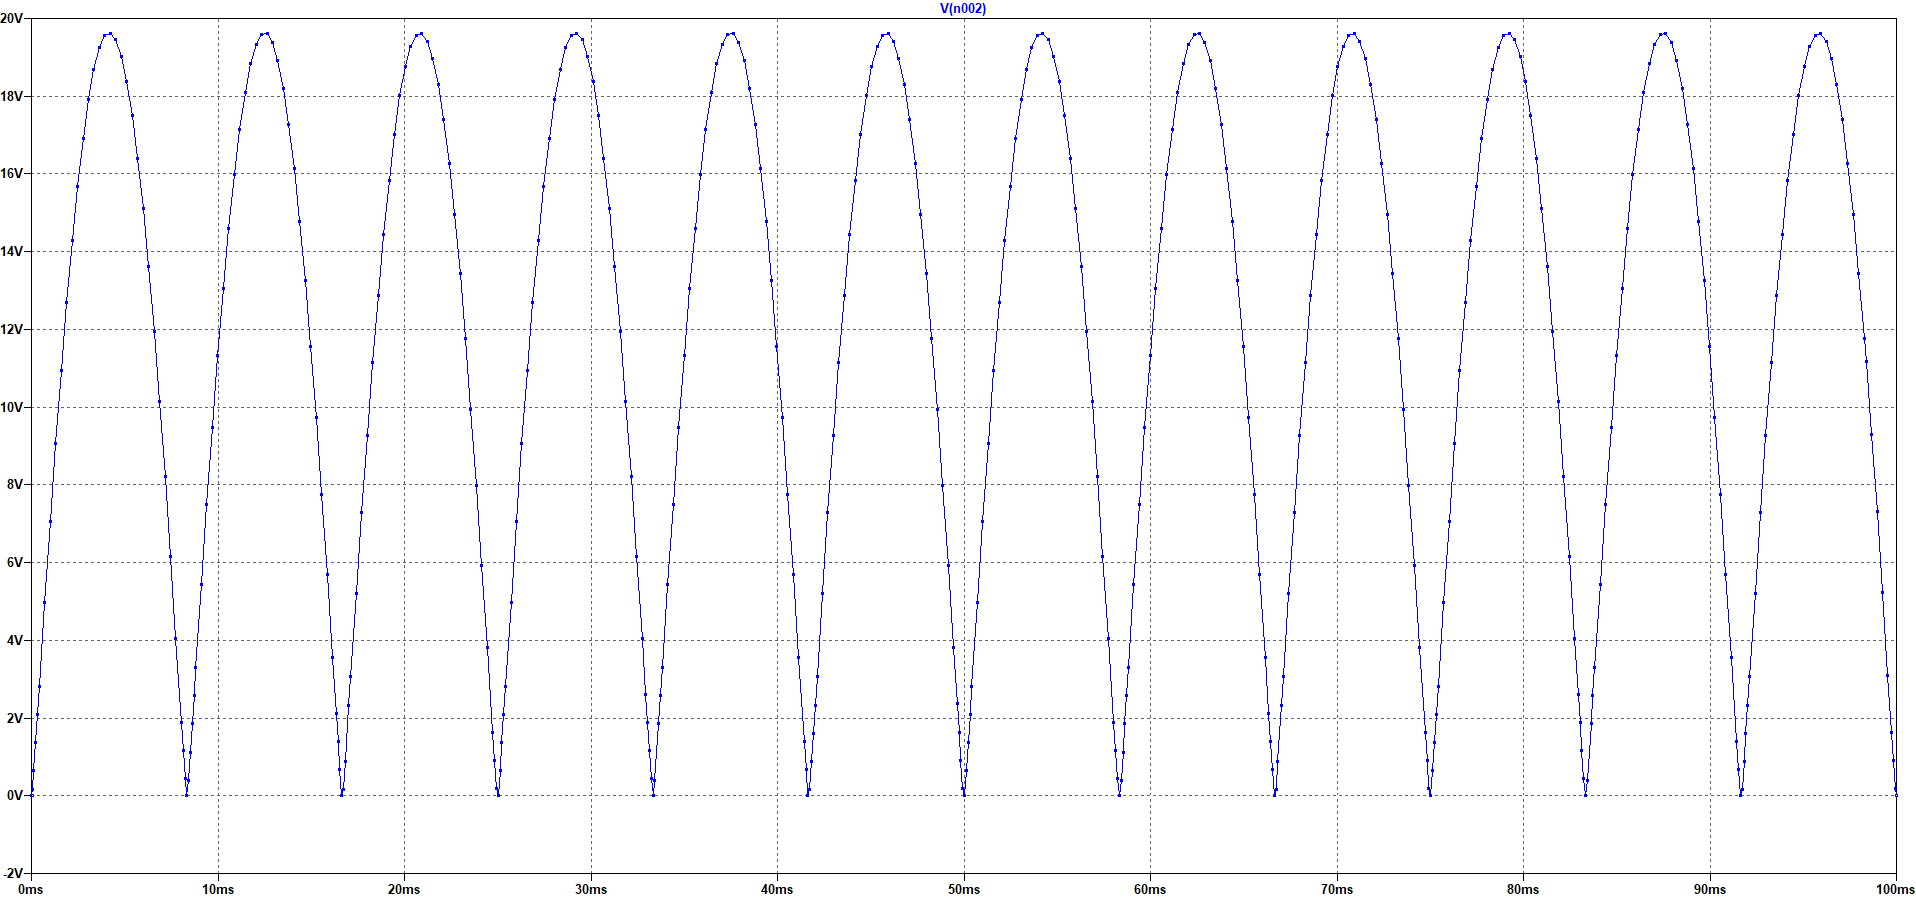
\includegraphics[width=0.70\textwidth]{Auxiliar_4_21}
  \caption{Bosquejo de \(v_o(t)\): rectificación de onda completa. Para \(v_i(t)=10\sin(\omega t)\,\text{V}\) ideal, los máximos de \(v_o\) alcanzan \(10\,\text{V}\) y los semiciclos negativos se reflejan hacia arriba.}
  \label{fig:voltaje-salida-4.1}
\end{figure}


    \subsection*{Resolucion 4.2}
  De manera análoga al caso anterior, analizamos el circuito con diodos ideales (\(V_\gamma=0\)) por casos según el signo de \(v_i\). En cada semiciclo, cada diodo se reemplaza por su modelo ON (corto) u OFF (abierto), como se muestra en las Figuras~\ref{fig:resolucion4.2a} y \ref{fig:resolucion4.2b}.

\begin{figure}[H]
  \centering
  \begin{subfigure}[b]{0.48\textwidth}
    \centering
    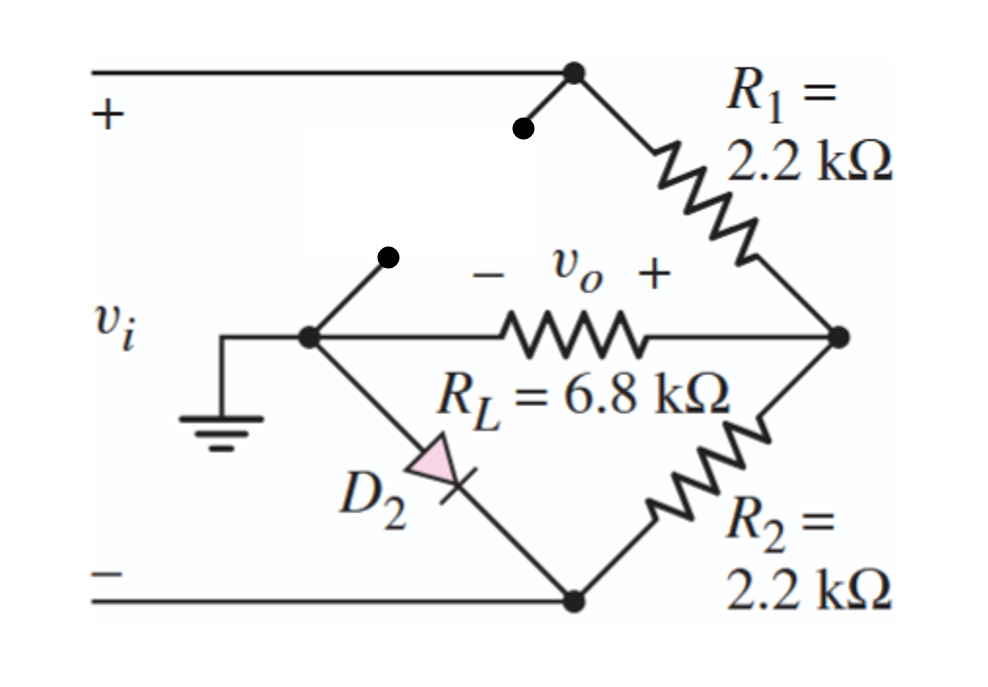
\includegraphics[width=\linewidth]{Auxiliar_4_23}
    \caption{\textbf{Caso 1:} \(v_i>0\). Conduce \(D_2\) (ON) y el otro diodo queda en OFF. El nodo \(v_o\) queda fijado por la fuente a través del corto ideal.}
    \label{fig:resolucion4.2a}
  \end{subfigure}\hfill
  \begin{subfigure}[b]{0.48\textwidth}
    \centering
    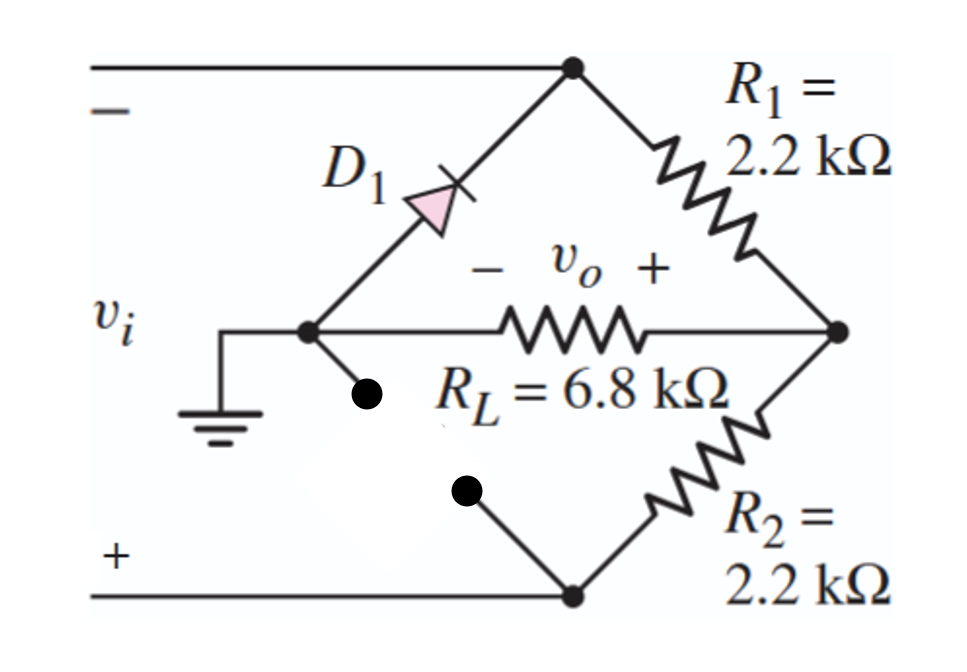
\includegraphics[width=\linewidth]{Auxiliar_4_24}
    \caption{\textbf{Caso 2:} \(v_i<0\). Conduce \(D_1\) (ON) y el otro diodo queda en OFF. Por simetría, el nodo \(v_o\) vuelve a quedar fijado por la fuente (con polaridad reflejada por el diodo).}
    \label{fig:resolucion4.2b}
  \end{subfigure}
  \caption{Modelo ON/OFF en cada semiciclo. En ambos casos, visto desde \(v_o\), el diagrama reducido es del mismo tipo: el diodo conductor “pega” \(v_o\) a la fuente; el diodo bloqueado aísla la rama opuesta.}
  \label{fig:resolucion4.2}
\end{figure}

Para facilitar el análisis, es útil \emph{etiquetar nodos} y reordenar el circuito sin cambiar conexiones. Con lo que se obtiene lo visto en \ref{fig:equivalente-vo-2}
\begin{figure}[H]
  \centering
  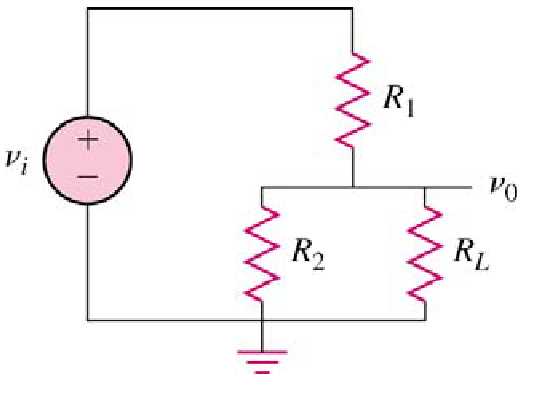
\includegraphics[width=0.44\textwidth]{Auxiliar_4_25}
  \caption{Esquema equivalente desde \(v_o\) (válido en ambos semiciclos). El diodo que conduce fija \(v_o\) al valor instantáneo de la fuente; la rama opuesta queda aislada.}
  \label{fig:equivalente-vo-2}
\end{figure}

Por lo que por la simetría de la red y el modelo ideal de los diodos, el circuito realiza una \textbf{rectificación de onda completa}:
\[
  v_o(t)=|\,v_i(t)\,|.
\]
Es decir, \(v_o\) sigue el valor absoluto de la fuente: los semiciclos negativos se reflejan hacia arriba.

\begin{figure}[H]
  \centering
  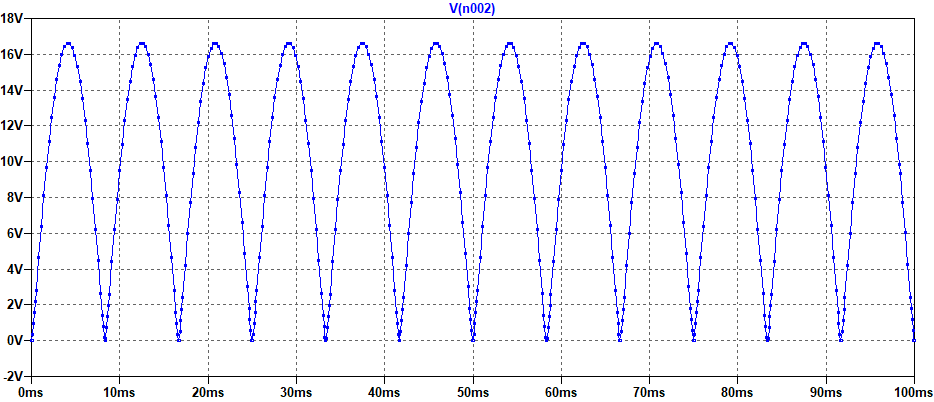
\includegraphics[width=0.80\textwidth]{Auxiliar_4_26}
  \caption{Bosquejo/simulación de \(v_o(t)\): rectificación de onda completa (picos iguales a los de \(v_i\) si el diodo es ideal).}
  \label{fig:voltaje-salida-4.2}
\end{figure}

\end{solution}
\end{questions}
\end{document}